% No compression; prevents errors when viewing PDF on Windows
\pdfobjcompresslevel=0

\documentclass[12pt]{article}

\usepackage{mathptmx,times}
\usepackage{amsmath}
\usepackage{tabularx}
\usepackage{booktabs, ragged2e, array, dcolumn}
\usepackage[font=small,format=plain,labelfont=bf,up]{caption}
\usepackage[bookmarks,hidelinks]{hyperref} % Enables table of content in PDF viewers; hide link boxes

\setlength{\textwidth}{6.5in}
\setlength{\textheight}{8.5in}
\setlength{\topmargin}{0in}
\setlength{\headheight}{0.25in}
\setlength{\headsep}{0.5in}
\setlength{\oddsidemargin}{0in}
\setlength{\evensidemargin}{0.0in}
\setlength{\voffset}{-0.4in}
\setlength{\footskip}{0.5in}
\setlength{\marginparpush}{7pt}
\setlength{\parskip}{\baselineskip}
\setlength{\parindent}{0pt}

\usepackage{titlesec}
\usepackage{graphicx}
\usepackage{floatrow}

\usepackage{lineno}

\titlelabel{\thetitle.\quad}
\titleformat*{\section}{\bf\normalsize}
\titleformat*{\subsection}{\bf\normalsize}
\titlespacing\section{0pt}{12pt plus 4pt minus 2pt}{0pt plus 2pt minus 2pt}
\titlespacing\subsection{0pt}{12pt plus 4pt minus 2pt}{0pt plus 2pt minus 2pt}
\titlespacing\subsubsection{0pt}{12pt plus 4pt minus 2pt}{0pt plus 2pt minus 2pt}

\begin{document}

\begin{flushright}
\textbf{PBNC2014-218}
\end{flushright}

\begin{center}
\textbf{COMBINED FIRE MODEL UNCERTAINTY AND INPUT PARAMETER UNCERTAINTY ANALYSIS FOR NUCLEAR POWER PLANT FIRE SCENARIOS}
% \textbf{A MONTE CARLO ANALYSIS OF THE EFFECT OF FIRE SEVERITY ON NUCLEAR SAFETY STRUCTURES, SYSTEMS, AND COMPONENTS}
\end{center}

\begin{center}
\textbf{K. Overholt\textsuperscript{1}, M. Clouthier\textsuperscript{2}}\\
\textsuperscript{1}National Institute of Standards and Technology, Gaithersburg, MD, USA\\
\textsuperscript{2}Fauske \& Associates, Nova Scotia, Canada
\end{center}

\begin{center}
\textbf{Abstract}
\end{center}

\linenumbers 
 
Quantitative fire risk analysis is used in conducting safety assessments at nuclear facilities to evaluate the potential consequences of postulated fire scenarios that can potentially damage nuclear safety structures, systems, and components. Some limitations exist when using point estimates or when conducting bounding analysis to determine pass/fail criteria for a given scenario. Specifically, these methods do not take into account probability distributions of input parameters. Therefore, in some cases, a more robust methodology for uncertainty analysis is needed, and the effect of different types of uncertainty should be considered in a quantitative analysis.

The purpose of this paper is to present an uncertainty analysis for a single fire scenario that accounts for different types of uncertainty. Three cases are presented that account for the effect of different types of uncertainty on the probability of exceeding a specified criterion: model bias and uncertainty, input parameter uncertainty, and a combination of model bias/uncertainty and input parameter uncertainty. For this uncertainty analysis, the heat release rate (HRR) was selected as the uncertain input parameter of interest, and the HGL temperature was selected as the model output quantity of interest. The Consolidated Model of Fire Growth and Smoke Transport (CFAST) zone model was used to predict hot gas layer temperatures for a given input HRR.

\section{Introduction}
\label{sec:introduction}
% !TEX root = PBNC_Paper.tex

The area of uncertainty analysis is well established in science and engineering \cite{Morgan}.  Its role is to provide insight on the impact of uncertainties associated with engineering evaluations, which allows for meaningful and defensible decision making in risk assessment.

The practice of uncertainty analysis in fire modelling is evolving and the methodology employed is currently left to the practitioners' discretion. Often, a bounding analysis approach is taken, based on the assumption that uncertainty is addressed by specifying conservative values for input parameters. In some cases, bounding analysis by adopting a series of conservative assumptions as a substitute for uncertainty analysis could result in overly conservative decisions or provide a false understanding of the actual margin of safety. 

Uncertainty is addressed in fire protection engineering literature \cite{Notarianni:SFPE}.  And treatment of uncertainty analysis is explicitly required in most technical standards related to fire safety at nuclear power generating stations \cite{NFPA:805, NUREG:6850}.  Model bias and uncertainty has been quantified in Nuclear Regulatory Commission (NRC) NUREG-1824~\cite{NUREG_1824_Sup_1} for a number of fire models which are commonly used in nuclear power plant applications. This information can be used as part of a specific methodology to evaluate model uncertainty  that is presented in NRC NUREG-1934~\cite{NUREG_1934}. 

The treatment of  uncertainty and sensitivity in NUREG-1934 includes a summary of a derivation for quantifying model uncertainty \cite{McGrattan2011a}, as well as specific calculation examples in Section 4.3. Parameter uncertainty and methods to deal with this kind of uncertainty are discussed separately in Section 4.4; a simple brute force method is shown in  a worked example that propagates a HRR distribution through an algebraic model for predicted flame height, and determines the probability of flames reaching a certain height.

Given that input parameter uncertainty and model uncertainty are a both addressed separately in NUREG-1934; an apparent logical extension of the methodologies presented would be to treat both kinds of uncertainty in a manner that shows the combined effect of both kinds of uncertainty.  It is the aim of this paper to provide practitioners with a straight-forward and practical example of combined model and input uncertainty uncertainty analysis for a zone fire modelling application. 

In this paper, we demonstrate the calculation of three cases for one worked example for a fire scenario that is typical for a nuclear power generating station: 1) the effect of model bias and uncertainty, 2) the effect of input parameter uncertainty, and 3) the combined effect of model bias/uncertainty and input parameter uncertainty. 



\section{Previous work}
\label{sec:previous_work}

% !TEX root = PBNC_Paper.tex

The subject of model uncertainty and input parameter uncertainty and sensitivity has been covered extensively in the literature \cite{Spiegel, Vose, Kumamoto, Haimes}.  And there are numerous studies specific to fire modelling \cite{Notarianni:SFPE,  NUREG_1824, McGrattan2011a, Notarianni:1999, Lundin, Hostikka:2003a, Upadhyay2008, FDS_Validation_Guide}.  

Researchers have explored different methods for assessing uncertainty and sensitivity in complex models. In terms of sensitivity of output parameters to input values, Iman and Helton \cite{Iman:1988} concluded that Monte Carlo sampling offered the best overall performance compared to other methods such as differential analysis or response surface replacements.

Hostikka and Rahkonen \cite{Hostikka:2003a} used Monte Carlo simulation and CFAST to evaluate model sensitivity to numerous  input parameters such as fire power and growth rate, compartment geometry, and ventilation. This work estimated probabilities in terms of time to failure of electric cables in a tunnel fire, and hot gas layer development  in a compartment due to an electrical cabinet fire. 

A technique for calculating the sensitivity in model outputs resulting  from input parameter uncertainty is provided in Volume 2 of NUREG-1824. This method, which is also described in the Fire Dynamics Simulator (FDS) Technical Reference Guide \cite{FDS_Validation_Guide}, involves quantifying the functional dependence of the input parameters, based on the governing mathematical equations or simple algebraic correlations. 

A method for calculating model uncertainty is derived by McGrattan and Toman \cite{McGrattan2011a} and summarized in \cite{FDS_Validation_Guide}. This method involves comparisons of model predictions with experimental measurements. The work by McGrattan and Toman \cite{McGrattan2011a} presents a derivation of formulae to calculate  a bias factor and a relative standard deviation for a given model. Key assumptions are: (1) Experimental measurements are normally distributed about the ``true'' values, and there is no associated experimental systematic bias; and, (2)  model predictions are normally distributed about the true values multiplied by a bias factor. This methodology was applied for a number of fire models and the results of the study are presented in NUREG-1824.

In this work, the approach taken to evaluate the affect of model uncertainty follows the method developed by McGrattan and Toman and uses the results provided for CFAST in NUREG-1824 \cite{NUREG_1824_Sup_1}. The Monte Carlo method was used to evaluate model input parameter uncertainty for a single parameter. This paper presents a worked example of model and input parameter uncertainty analysis for a consistent fire scenario at a  nuclear power plant.  Initially, input parameter and model uncertainty are considered separately. Then, a combined approach is taken where both kinds of uncertainty are treated together.
 
 
 

 
 
 
 
 







\section{Fire model scenario and computational setup}
\label{sec:fire_model_scenario_setup}

For this uncertainty analysis, the Consolidated Model of Fire Growth and Smoke Transport (CFAST) zone model~\cite{CFAST_Users_Guide_6} version 6.3.0 (SVN revision number 1462) was used to predict hot gas layer (HGL) temperatures for a given input heat release rate (HRR). The ``Cabinet Fire in Switchgear Room'' scenario in Appendix~B of NRC NUREG-1934~\cite{NUREG_1934} was selected for this uncertainty analysis. The compartment had dimensions of 26.5~m by 18.5~m by 6.1~m. The ambient temperature was specified as 20~$^\circ$C. The simulation time was 1~h (3600~s). The ceiling, wall, and floor materials were specified as concrete with a thickness of 0.5~m and a thermal conductivity of 1.6~W/m-K, density of 2400~kg/m$^3$, and specific heat of 0.75~J/g-K.

The HRR was selected as the uncertain input parameter of interest, and the distribution of HRRs is described in more detail in the following section. The HGL temperature was selected as the model output quantity of interest. The fuel properties were the same as the NRC NUREG-1934 Appendix~B example case: polyethylene (PE) insulated, polyvinyl chloride (PVC) jacketed cables with a heat of combustion of 20,900~kJ/kg, soot yield of 0.136~kg/kg, carbon monoxide yield of 0.147~kg/kg, and radiative fraction of 0.49.

For the uncertainty analysis, the Python programming language was used as a wrapper to automate CFAST model runs, collect the output from the CFAST model, run the Monte Carlo simulation, calculate probabilities of exceeding the threshold temperature, and generate the plots. Python is a high-level, flexible, and powerful programming language that is well-suited to scientific and engineering applications~\cite{Oliphant:2007}. Additional modules that were used with Python include NumPy~\cite{oliphant2006guide}, SciPy~\cite{Jones:2001fk}, and matplotlib~\cite{Hunter:2007}. The source code of the scripts that were used for these examples is open source and freely available for download.\footnote{\url{https://code.google.com/p/fire-tools/}}


\section{Uncertainty analysis}
\label{sec:uncertainty_analysis}

 To simplify this uncertainty analysis and to present a concise example, the HRR was selected as the only uncertain model input parameter. The other input parameters were considered to be fixed scenario parameters. In reality, there is some amount of uncertainty associated with the other input parameters. The HRR was held constant throughout the simulation. For the probability distribution of the HRR input parameter, a gamma distribution from NRC NUREG-6850~\cite{NUREG_6850} was selected, which has a 75th percentile HRR of 232~kW and a 98th percentile HRR of 1002~kW. This distribution has a shape parameter $\alpha$ of 0.46 and a scale parameter $\beta$ of 386. This corresponds to the HRR distribution of vertical cabinets with unqualified cable, fire in more than one cable bundle, with open doors. The HGL temperature was selected as the model output quantity of interest. A threshold (or critical) HGL temperature of 100~$^\circ$C was selected for this analysis, and the results included a calculation of the probability of exceeding this threshold HGL temperature.

The following sections present three cases that account for the effect of different types of uncertainty on the probability of exceeding the threshold HGL temperature. Case~1 accounts for the effect of model bias and uncertainty, Case~2 accounts for the effect of input parameter uncertainty, and Case~3 accounts for the combined effect of model bias/uncertainty and input parameter uncertainty. For Case~1, a HRR of 1002~kW is considered, which corresponds to the the 98th percentile HRR value of the gamma distribution. For Cases 2 and 3, the gamma distribution is used directly.



\clearpage


\subsection{Case 1: Effect of model bias and uncertainty}

This case accounts for the effect of model bias and uncertainty on the probability of exceeding the threshold HGL temperature. A HRR of 1002~kW was selected as the input fire size, which represents the 98th percentile HRR value of the gamma distribution. The probability density function (PDF) and cumulative distribution function (CDF) of the input HRR distribution are shown in Fig.~\ref{fig:case_1_input_distributions}. The probability of exceeding the threshold HGL temperature can be calculated following the procedure described in Section~4.3 (``Calculation of Model Uncertainty'') of NRC NUREG-1934~\cite{NUREG_1934}.

\textbf{Step 1}: Specify the input HRR and run CFAST to calculate the resulting HGL temperature.

For an input HRR of 1002~kW, the CFAST model predicts an HGL temperature of 90.7~$^\circ$C at a time of 3600~s (1 h).

\textbf{Step 2}: Subtract the ambient value of the HGL temperature (20~$^\circ$C) to determine the predicted temperature rise as
\begin{equation}
M = 90.7~^\circ\textrm{C} - 20~^\circ\textrm{C} = 70.7~^\circ\textrm{C}
\end{equation}

\textbf{Step 3}: Calculate the mean and standard deviation of the HGL temperature distribution.

Refer to Table 5-1 of NRC NUREG-1824 Supplement 1~\cite{NUREG_1824_Sup_1}, which indicates that, on average, CFAST overpredicts HGL temperatures in forced ventilation scenarios with a model bias factor $\delta$ of 1.15. The adjusted model prediction of the HGL temperature is calculated as
\begin{equation}
\mu = \frac{M}{\delta} = \frac{70.7~^\circ\textrm{C}}{1.15} \approx 81.5~^\circ\textrm{C}
\end{equation}
Refer again to Table 5-1 of NRC NUREG-1824 Supplement 1~\cite{NUREG_1824_Sup_1}, which indicates that the model relative standard deviation $\widetilde\sigma_M$ is 0.20. The standard deviation of the resulting distribution is calculated as
\begin{equation}
\sigma = \widetilde\sigma_M \left( \frac{M}{\delta} \right) = 0.20 \left( \frac{70.7}{1.15} \right) \approx 12.3~^\circ\textrm{C}
\end{equation}
Figure~\ref{fig:case_1_output_distributions} shows the PDF and CDF of the resulting HGL temperature distribution.

\textbf{Step 4}: Calculate the probability that the actual HGL temperature will exceed 100~$^\circ$C as
\begin{equation}
\textrm{P}(T > 100~^\circ\textrm{C}) = \frac{1}{2} \textrm{erfc} \left( \frac{T - \mu}{\sigma \sqrt{2}} \right) = \frac{1}{2} \textrm{erfc} \left( \frac{100~^\circ\textrm{C} - 81.5~^\circ\textrm{C}}{12.3~^\circ\textrm{C} \sqrt{2}} \right) \approx 0.066
\end{equation}
For Case~1, the probability of exceeding the threshold HGL temperature of 100~$^\circ$C was calculated as 0.066. Note that this estimate is based only on model bias and uncertainty.


\clearpage


\begin{figure}[p]
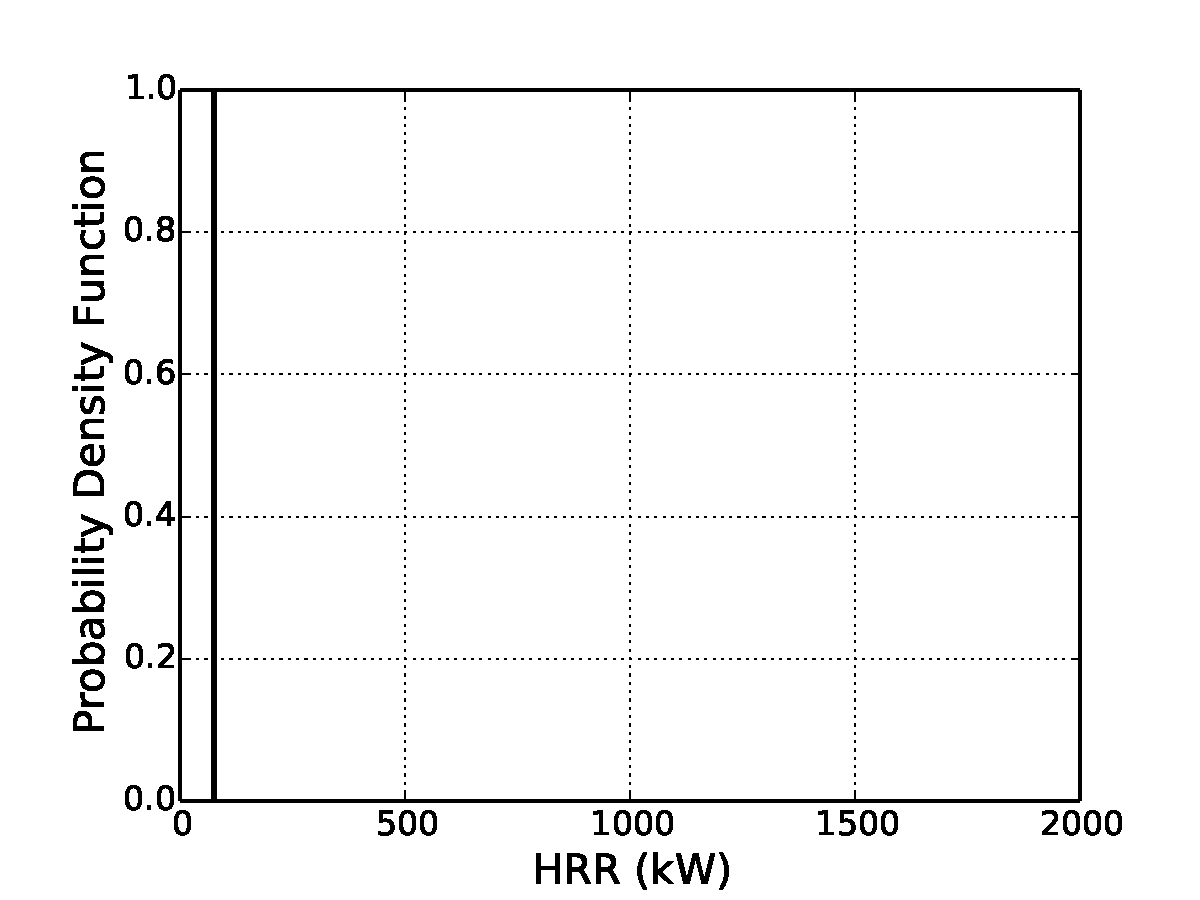
\includegraphics[width=3.2in]{Figures/input_PDF_point}
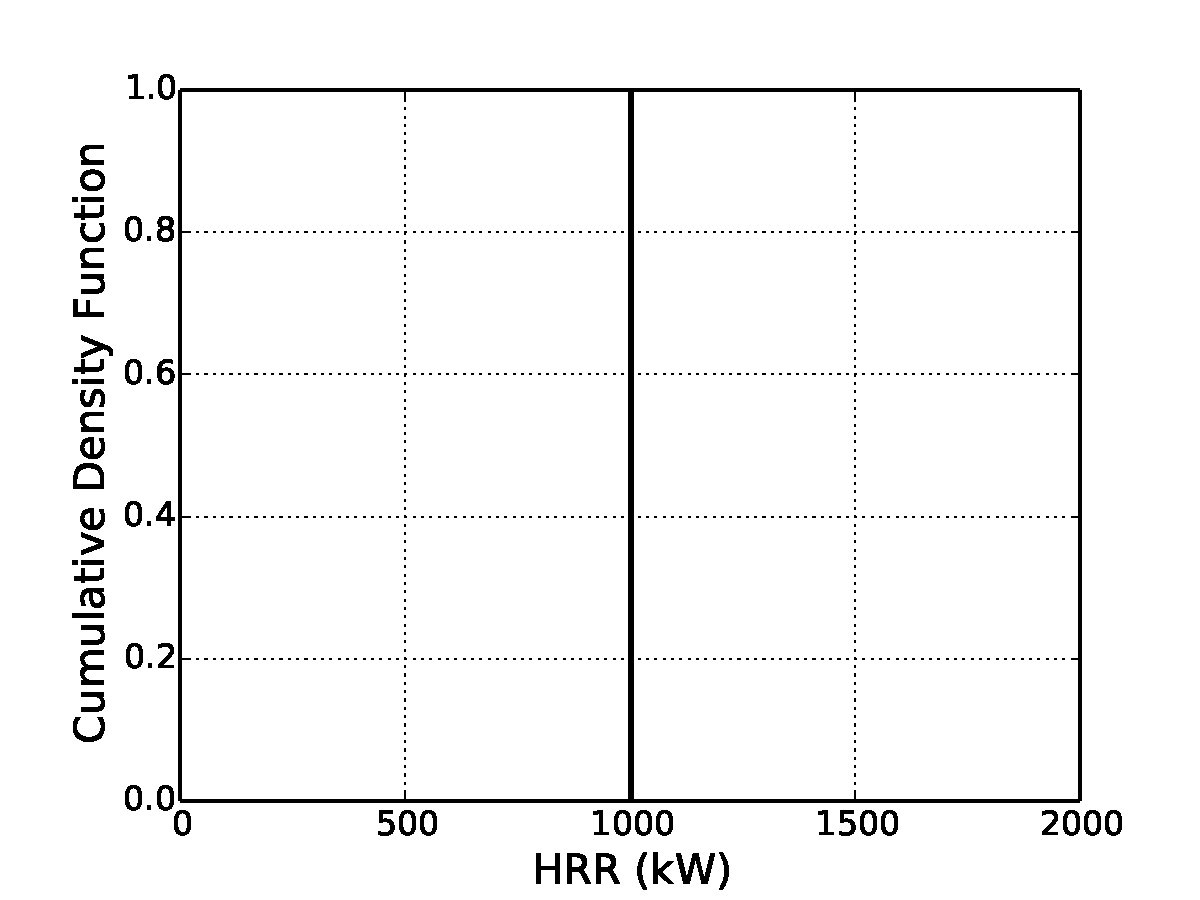
\includegraphics[width=3.2in]{Figures/input_CDF_point}
\caption{PDF and CDF of input HRR distribution for the case with model bias and uncertainty. This case used only one input HRR value, which corresponds to the 98th percentile HRR value of 1002~kW.}
\label{fig:case_1_input_distributions}
\end{figure}

\begin{figure}[p]
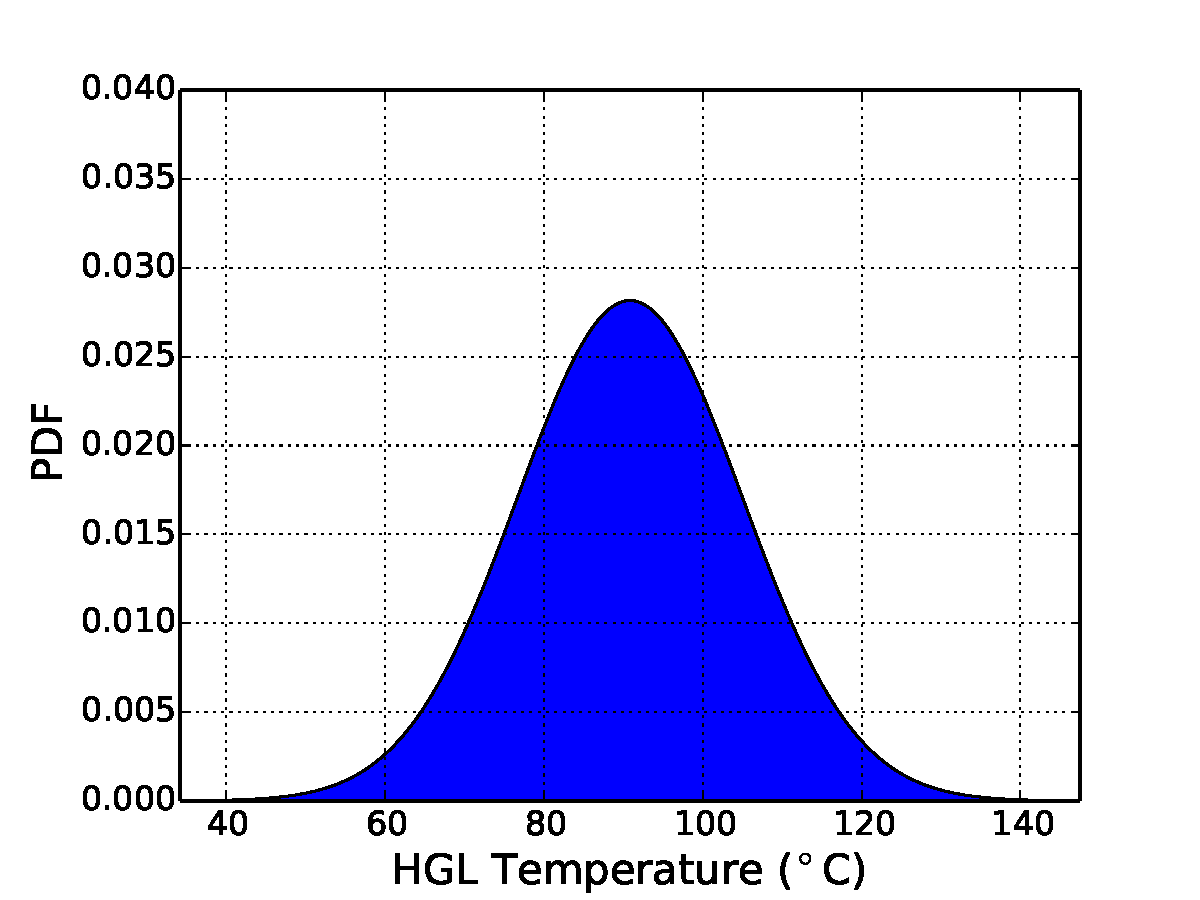
\includegraphics[width=3.2in]{Figures/output_PDF_1_model}
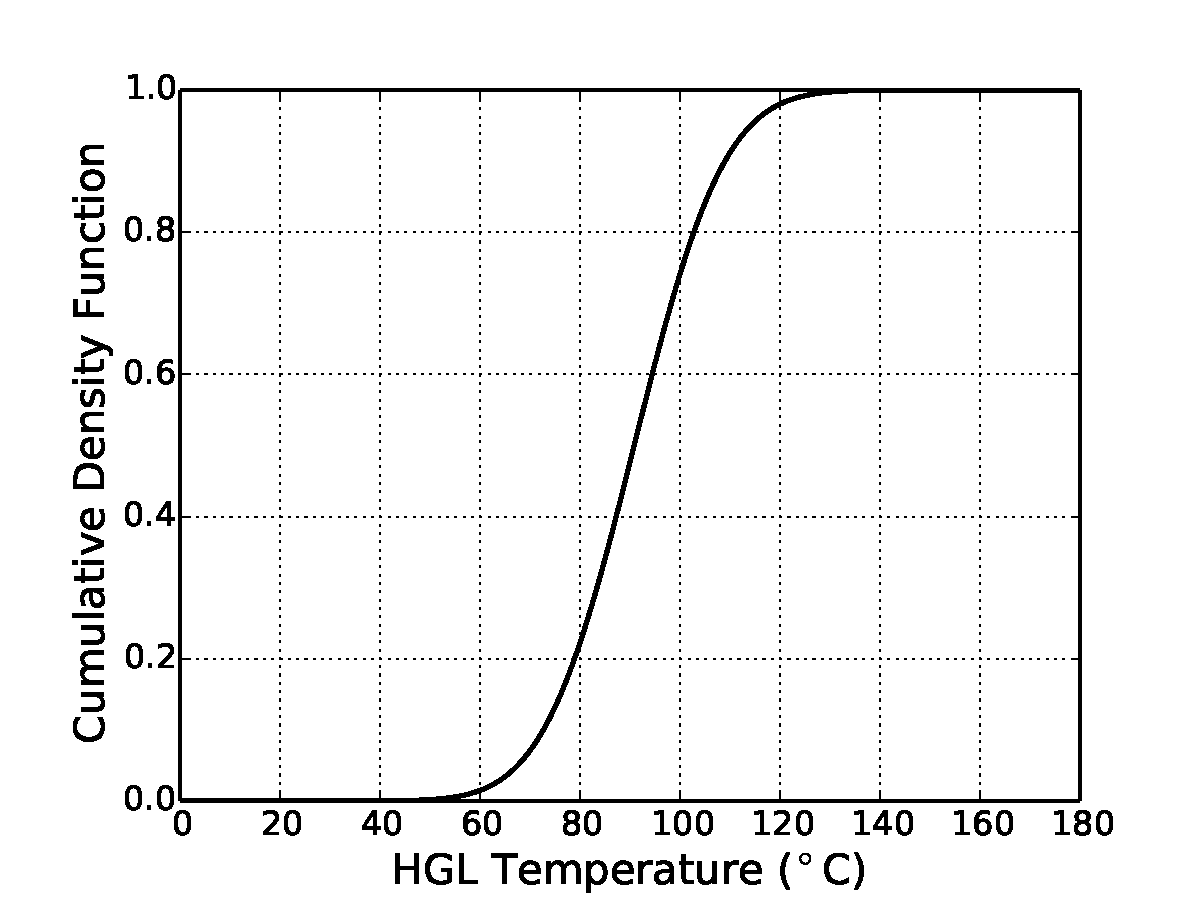
\includegraphics[width=3.2in]{Figures/output_CDF_1_model}
\caption{PDF and CDF of output HGL temperature distribution for the case with model bias and uncertainty. The vertical dashed line indicates the threshold HGL temperature of 100~$^\circ$C.}
\label{fig:case_1_output_distributions}
\end{figure}


\clearpage


\subsection{Case 2: Effect of input parameter uncertainty}

This case accounts for the effect of input parameter uncertainty on the probability of exceeding the threshold HGL temperature. The probability of exceeding the threshold HGL temperature can be calculated following the procedure described in Section 4.4.1 (``Parameter Uncertainty Propagation'') of NRC NUREG-1934~\cite{NUREG_1934}.

\textbf{Step 1}: Specify the input HRR distribution.

For the probability distribution of the HRR input parameter, a gamma distribution from NRC NUREG-6850~\cite{NUREG_6850} was selected, which has a 75th percentile HRR of 232~kW and a 98th percentile HRR of 1002~kW. This distribution has a shape parameter $\alpha$ of 0.46 and a scale parameter $\beta$ of 386. This corresponds to the HRR distribution of vertical cabinets with unqualified cable, fire in more than one cable bundle, with open doors. Other distributions could be used to represent the amount of uncertainty in the input parameter, such as a uniform or normal distribution, depending on the application and the amount of information that is available.

The Monte Carlo method was used to propagate the distribution of the input parameter (HRR) through the CFAST zone model to calculate the resulting distribution of the output quantity (HGL temperature). For this case, 50,000 Monte Carlo iterations were performed. The PDF and CDF of the input HRR distribution are shown in Fig.~\ref{fig:case_2_input_distributions}.

\textbf{Step 2}: Simulate the output HGL temperature distribution using the Monte Carlo method.

Draw a random sample from the input HRR distribution and run CFAST to calculate the HGL temperature. The HGL temperature value at a time of 3600~s (1 h) is stored. Step~2 is repeated to continue drawing samples from the input HRR distribution and calculating output HGL temperatures until the specified number of Monte Carlo iterations is reached.

Figure~\ref{fig:case_2_output_distributions} shows the PDF and CDF of the resulting HGL temperature distribution.

\textbf{Step 3}: Calculate the probability of exceeding the threshold HGL temperature.

Because the output HGL distribution was approximated using the Monte Carlo method, numerically integrate over the resulting distribution to calculate the probability of exceeding the threshold HGL temperature.

For Case~2, the probability of exceeding the threshold HGL temperature of 100~$^\circ$C was calculated as 0.012. Note that this estimate is based only on input parameter uncertainty.


\clearpage


\begin{figure}[p]
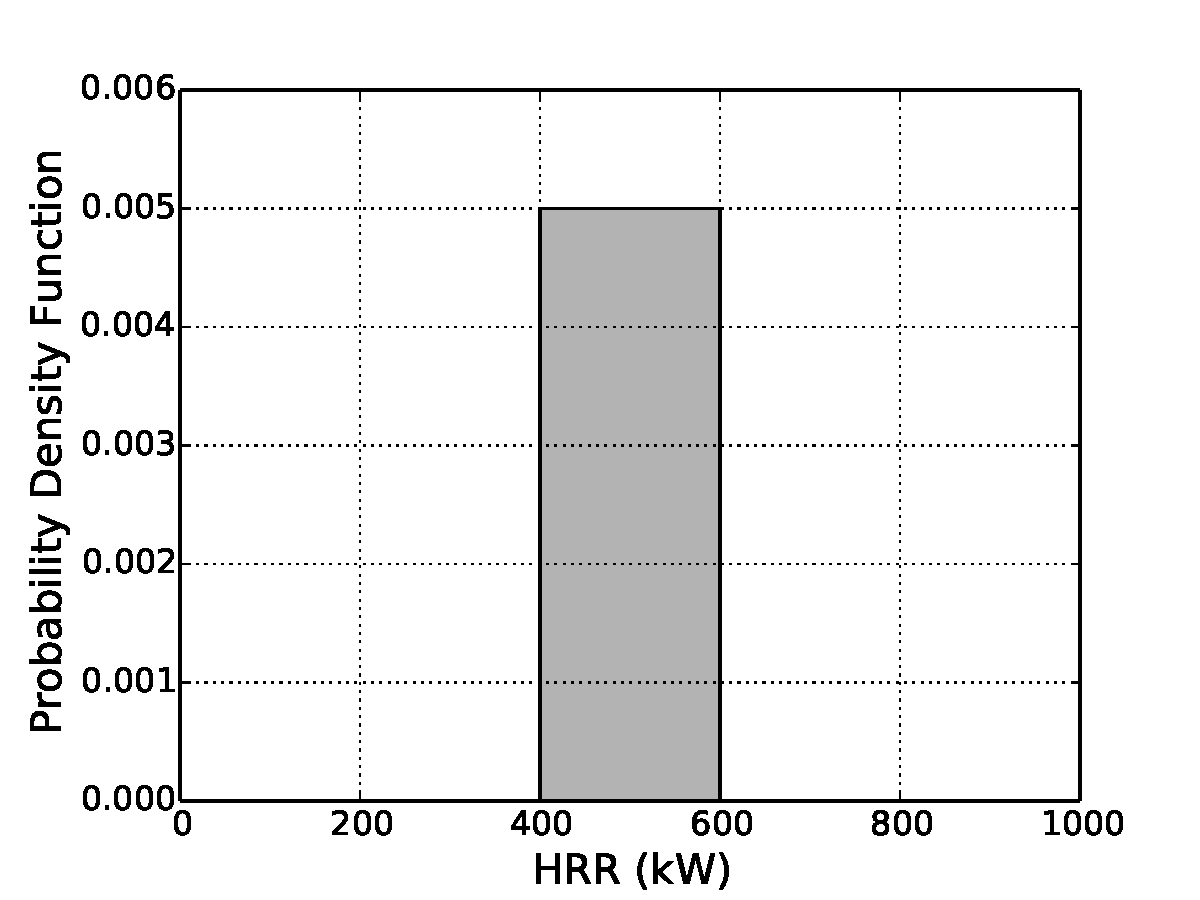
\includegraphics[width=3.2in]{Figures/input_PDF}
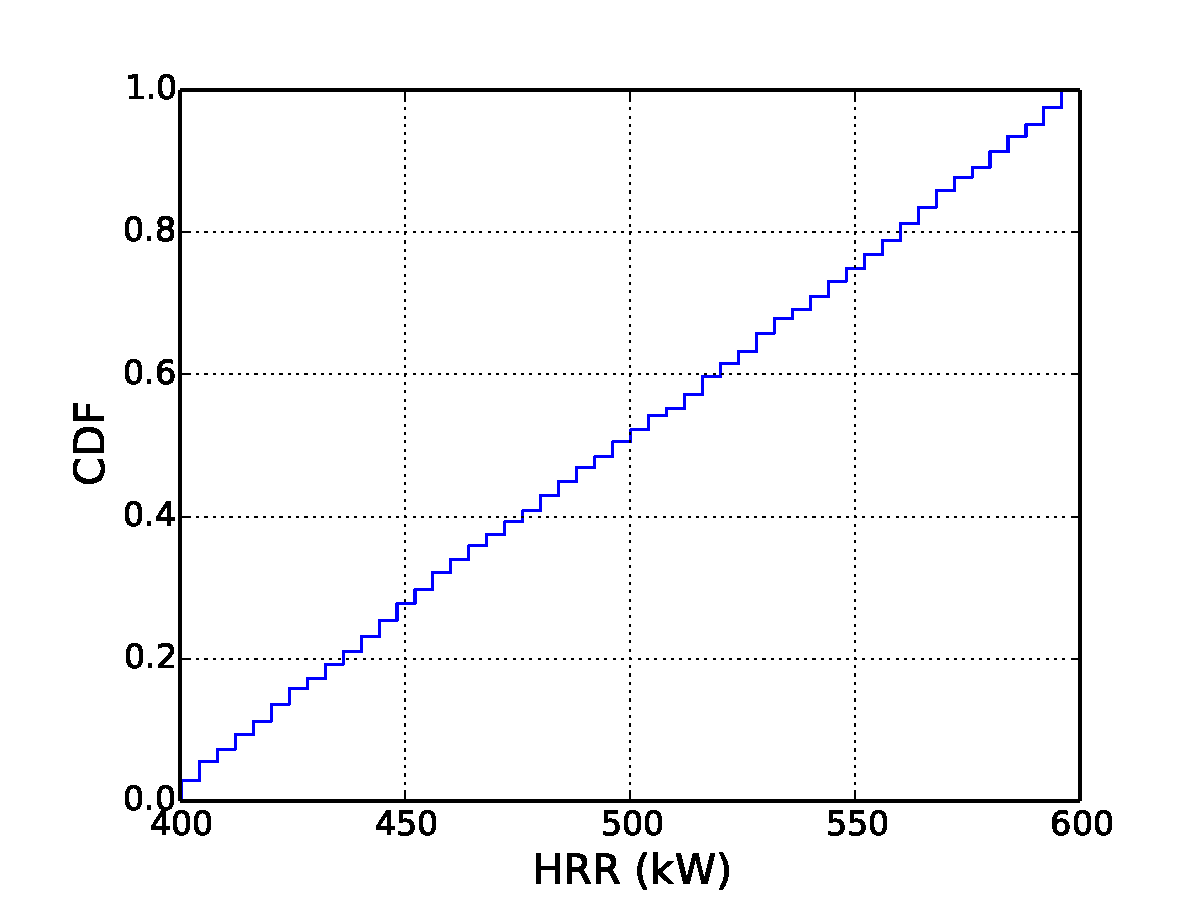
\includegraphics[width=3.2in]{Figures/input_CDF}
\caption{PDF and CDF of input HRR distribution for the case with input parameter uncertainty.}
\label{fig:case_2_input_distributions}
\end{figure}

\begin{figure}[p]
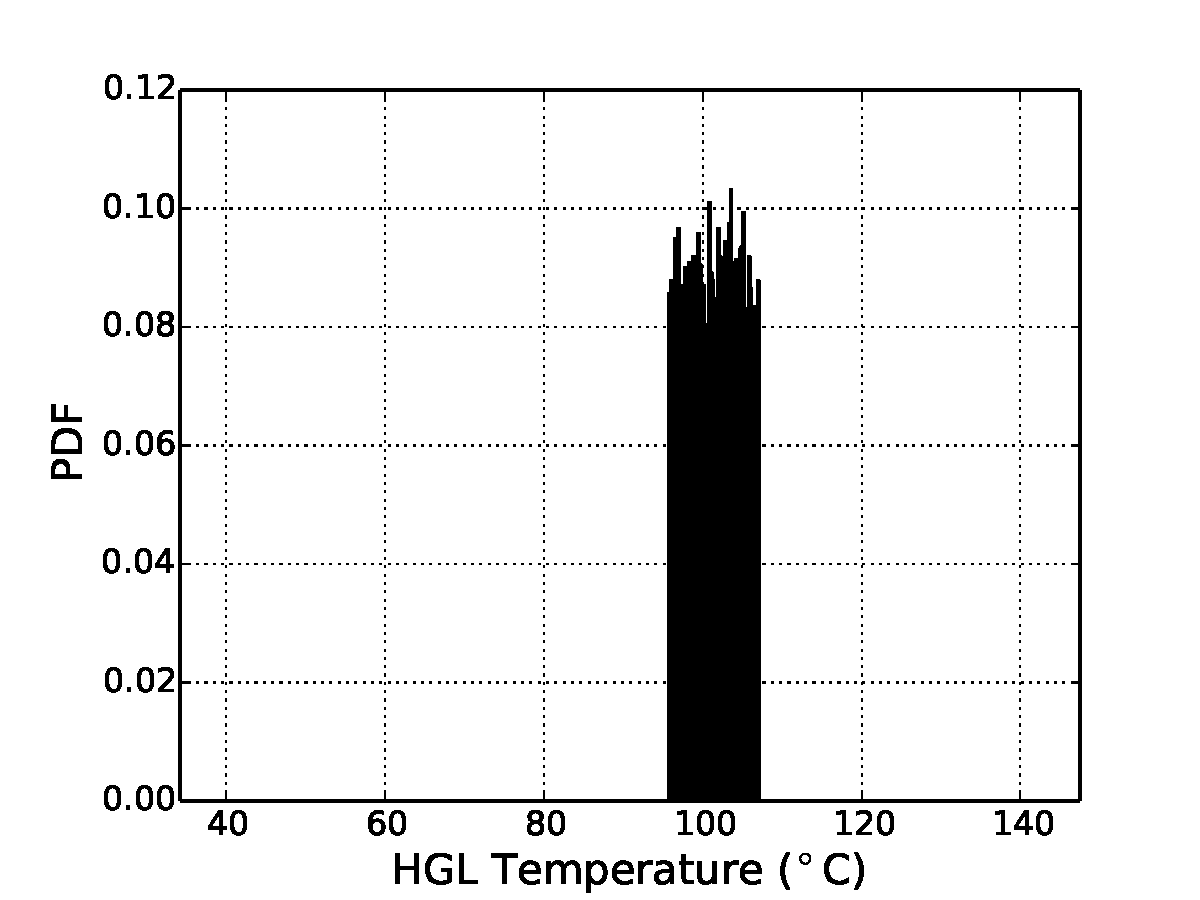
\includegraphics[width=3.2in]{Figures/output_PDF_2_input}
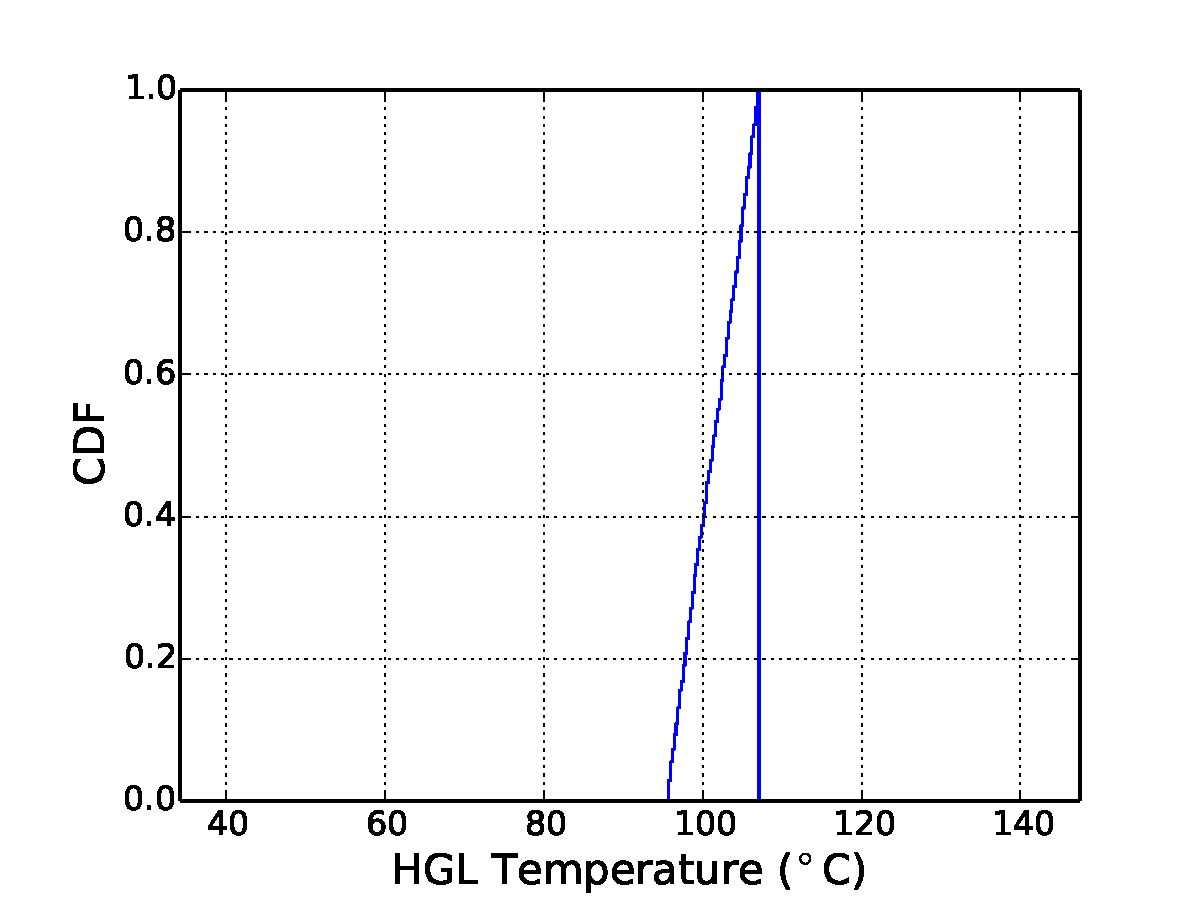
\includegraphics[width=3.2in]{Figures/output_CDF_2_input}
\caption{PDF and CDF of output HGL temperature distribution for the case with input parameter uncertainty. The vertical dashed line indicates the threshold HGL temperature of 100~$^\circ$C.}
\label{fig:case_2_output_distributions}
\end{figure}


\clearpage


\subsection{Case 3: Combined effect of model bias/uncertainty and input parameter uncertainty}

This case accounts for the combined effect of model bias/uncertainty and input parameter uncertainty on the probability of exceeding the threshold HGL temperature. Therefore, this case uses a combination of steps from Cases 1 and 2.

\textbf{Step 1}: Specify the input HRR distribution.

The probability distribution for the HRR input parameter was the same as in Case~2: a gamma distribution from NRC NUREG-6850~\cite{NUREG_6850} with a 75th percentile HRR of 232~kW and a 98th percentile HRR of 1002~kW. As in Case~2, 50,000 Monte Carlo iterations were performed. The PDF and CDF of the input HRR distribution are shown in Fig.~\ref{fig:case_3_input_distributions}.

\textbf{Step 2}: Draw a random sample from input HRR distribution and run CFAST to calculate the HGL temperature at 3600~s (1 h).

\textbf{Step 3}: For the resulting HGL temperature in Step~2, subtract the ambient value of the HGL temperature (20~$^\circ$C) to determine the predicted temperature rise.

\textbf{Step 4}: Calculate the mean and standard deviation of the HGL temperature distribution using the model bias factor $\delta$ of 1.15 and model relative standard deviation $\widetilde\sigma_M$ of 0.20 from Table 5-1 of NRC NUREG-1824 Supplement 1~\cite{NUREG_1824_Sup_1}.

\textbf{Step 5}: Draw a random HGL temperature value from the normal distribution that results from Step~4. This HGL temperature value is stored, then return to Step~2 to continue drawing samples from the HRR distribution until the specified number of Monte Carlo iterations is reached. Figure~\ref{fig:case_3_output_distributions} shows the PDF and CDF of the resulting HGL temperature distribution.

\textbf{Step 6}: Calculate the probability that the HGL temperature will exceed the threshold HGL temperature. Because the output HGL distribution was approximated using the Monte Carlo method, numerically integrate over the resulting distribution to calculate the probability of exceeding the threshold HGL temperature.

For Case~3, the probability of exceeding the threshold HGL temperature of 100~$^\circ$C was calculated as 0.008. Note that this estimate is based on the combined effect of model bias/uncertainty and input parameter uncertainty.


\clearpage


\begin{figure}[p]
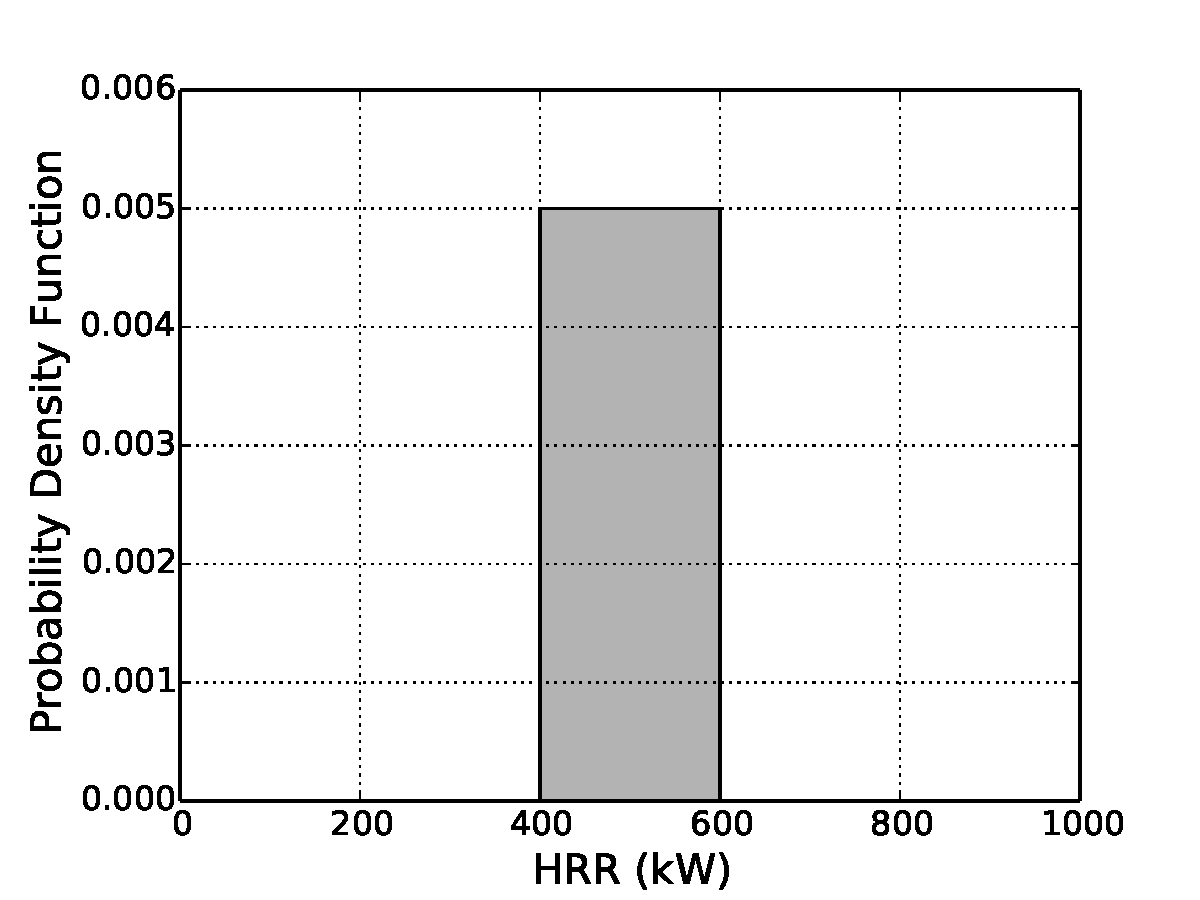
\includegraphics[width=3.2in]{Figures/input_PDF}
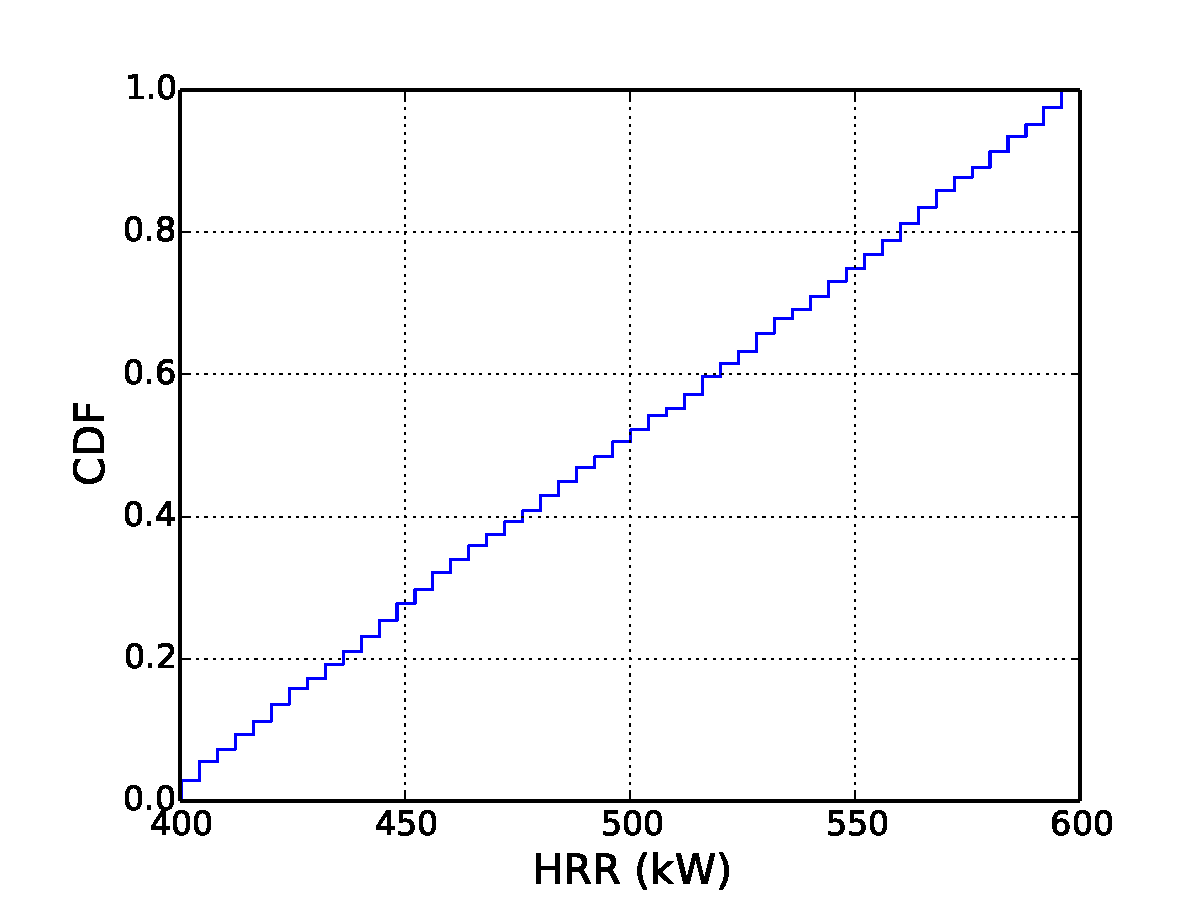
\includegraphics[width=3.2in]{Figures/input_CDF}
\caption{PDF and CDF of input HRR distribution for the case with combined model bias/uncertainty and input parameter uncertainty.}
\label{fig:case_3_input_distributions}
\end{figure}

\begin{figure}[p]
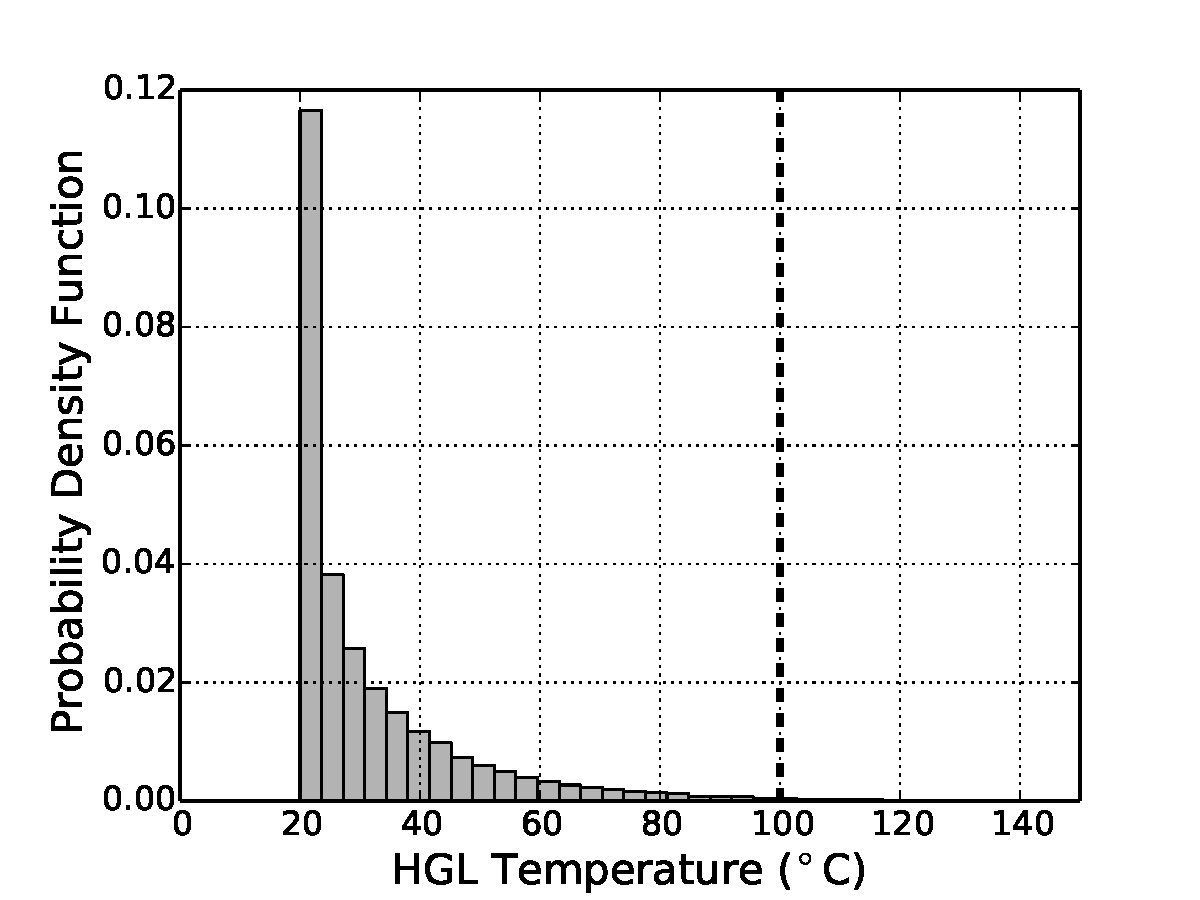
\includegraphics[width=3.2in]{Figures/output_PDF_3_combined}
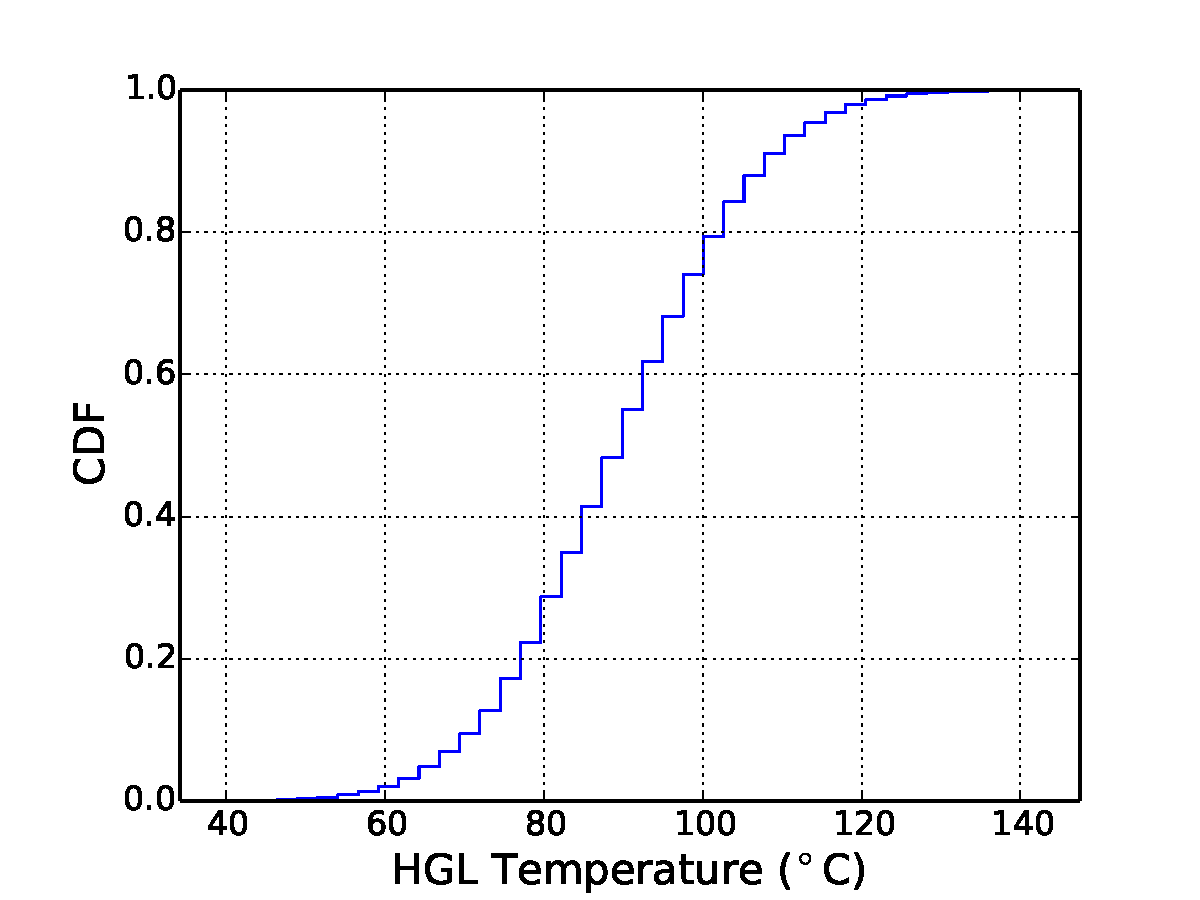
\includegraphics[width=3.2in]{Figures/output_CDF_3_combined}
\caption{PDF and CDF of output HGL temperature distribution for the case with combined model bias/uncertainty and input parameter uncertainty. The vertical dashed line indicates the threshold HGL temperature of 100~$^\circ$C.}
\label{fig:case_3_output_distributions}
\end{figure}


\clearpage


\section{Conclusions}
\label{sec:conclusions}

Three cases were presented that account for the effect of different types of uncertainty on the probability of exceeding the threshold HGL temperature. Case~1 accounted for the effect of model bias and uncertainty, Case~2 accounted for the effect of input parameter uncertainty, and Case~3 accounted for the combined effect of model bias/uncertainty and input parameter uncertainty. The probabilities of exceeding the threshold HGL temperature of 100~$^\circ$C were 0.066, 0.012, and 0.008 for Cases 1, 2, and 3, respectively.

Although Cases~2 and 3 used the same input HRR distribution, the probability in Case~3 was less than the probability in Case~2. This is most likely due to the model bias factor that was greater than 1, which tends to shift the adjusted model predictions to a lower HGL temperature value. Note that these results are scenario dependent and are not to be considered representative of a general uncertainty analysis. The purpose of this uncertainty analysis was to demonstrate the effect of different types of uncertainty (model uncertainty, input parameter uncertainty, and combined uncertainty) on the calculated probability. The use of probability distributions in uncertainty analyses allows for a more thorough examination of the impact of the choice of input parameters on the model predictions.


\bibliographystyle{unsrt}
\bibliography{references_ko,references_mpc}

\end{document}